% Standard 10pt
\documentclass[a4paper,twoside, openright]{scrartcl}

\usepackage[utf8]{inputenc}
\usepackage{fontspec, emptypage}
\usepackage[a4paper, left=2.5cm, right=2.5cm, bottom=2.8cm, top=2.8cm]{geometry}
\usepackage[ngerman,english]{babel}
\usepackage{fancyhdr, graphicx, amsmath, hyperref, longtable, float, enumitem, blindtext}
% For Bibliography
\usepackage{natbib}
\bibliographystyle{authordate1}
% For Abkürzungsverzeichnis
\usepackage{acronym}
% For appendix
\usepackage[toc,page]{appendix}
% For tikz
\usepackage{calc, ifthen, tikz}
% For including pdfs
\usepackage{pdfpages}
% Caption setup
\usepackage[tableposition=b]{caption}
\captionsetup[longtable]{skip=1em}
% Important for longtable
\usepackage{arydshln}

\hypersetup{
	colorlinks,
	citecolor=black,
	filecolor=black,
	linkcolor=black,
	urlcolor=black
}

\renewcommand{\baselinestretch}{1.2}
\newcommand{\tabitem}{~~\llap{\textbullet}~~}
\newcommand{\HRule}{\rule{\linewidth}{0.3mm}} % Defines a new command for the horizontal lines, change thickness here

\addto\captionsngerman{\let\appendixtocname\appendixname%
	\let\appendixpagename\appendixname}

\title{Bachelor Thesis}

\parindent 0pt

\begin{document}

% ----------------------------------------
% Titelblatt
% ----------------------------------------
\begin{titlepage}
\begingroup
\centering
\vspace*{\baselineskip}

\thispagestyle{empty}

\begin{figure}[H]
	\centering
	\begin{minipage}{.49\textwidth}
		\centering
		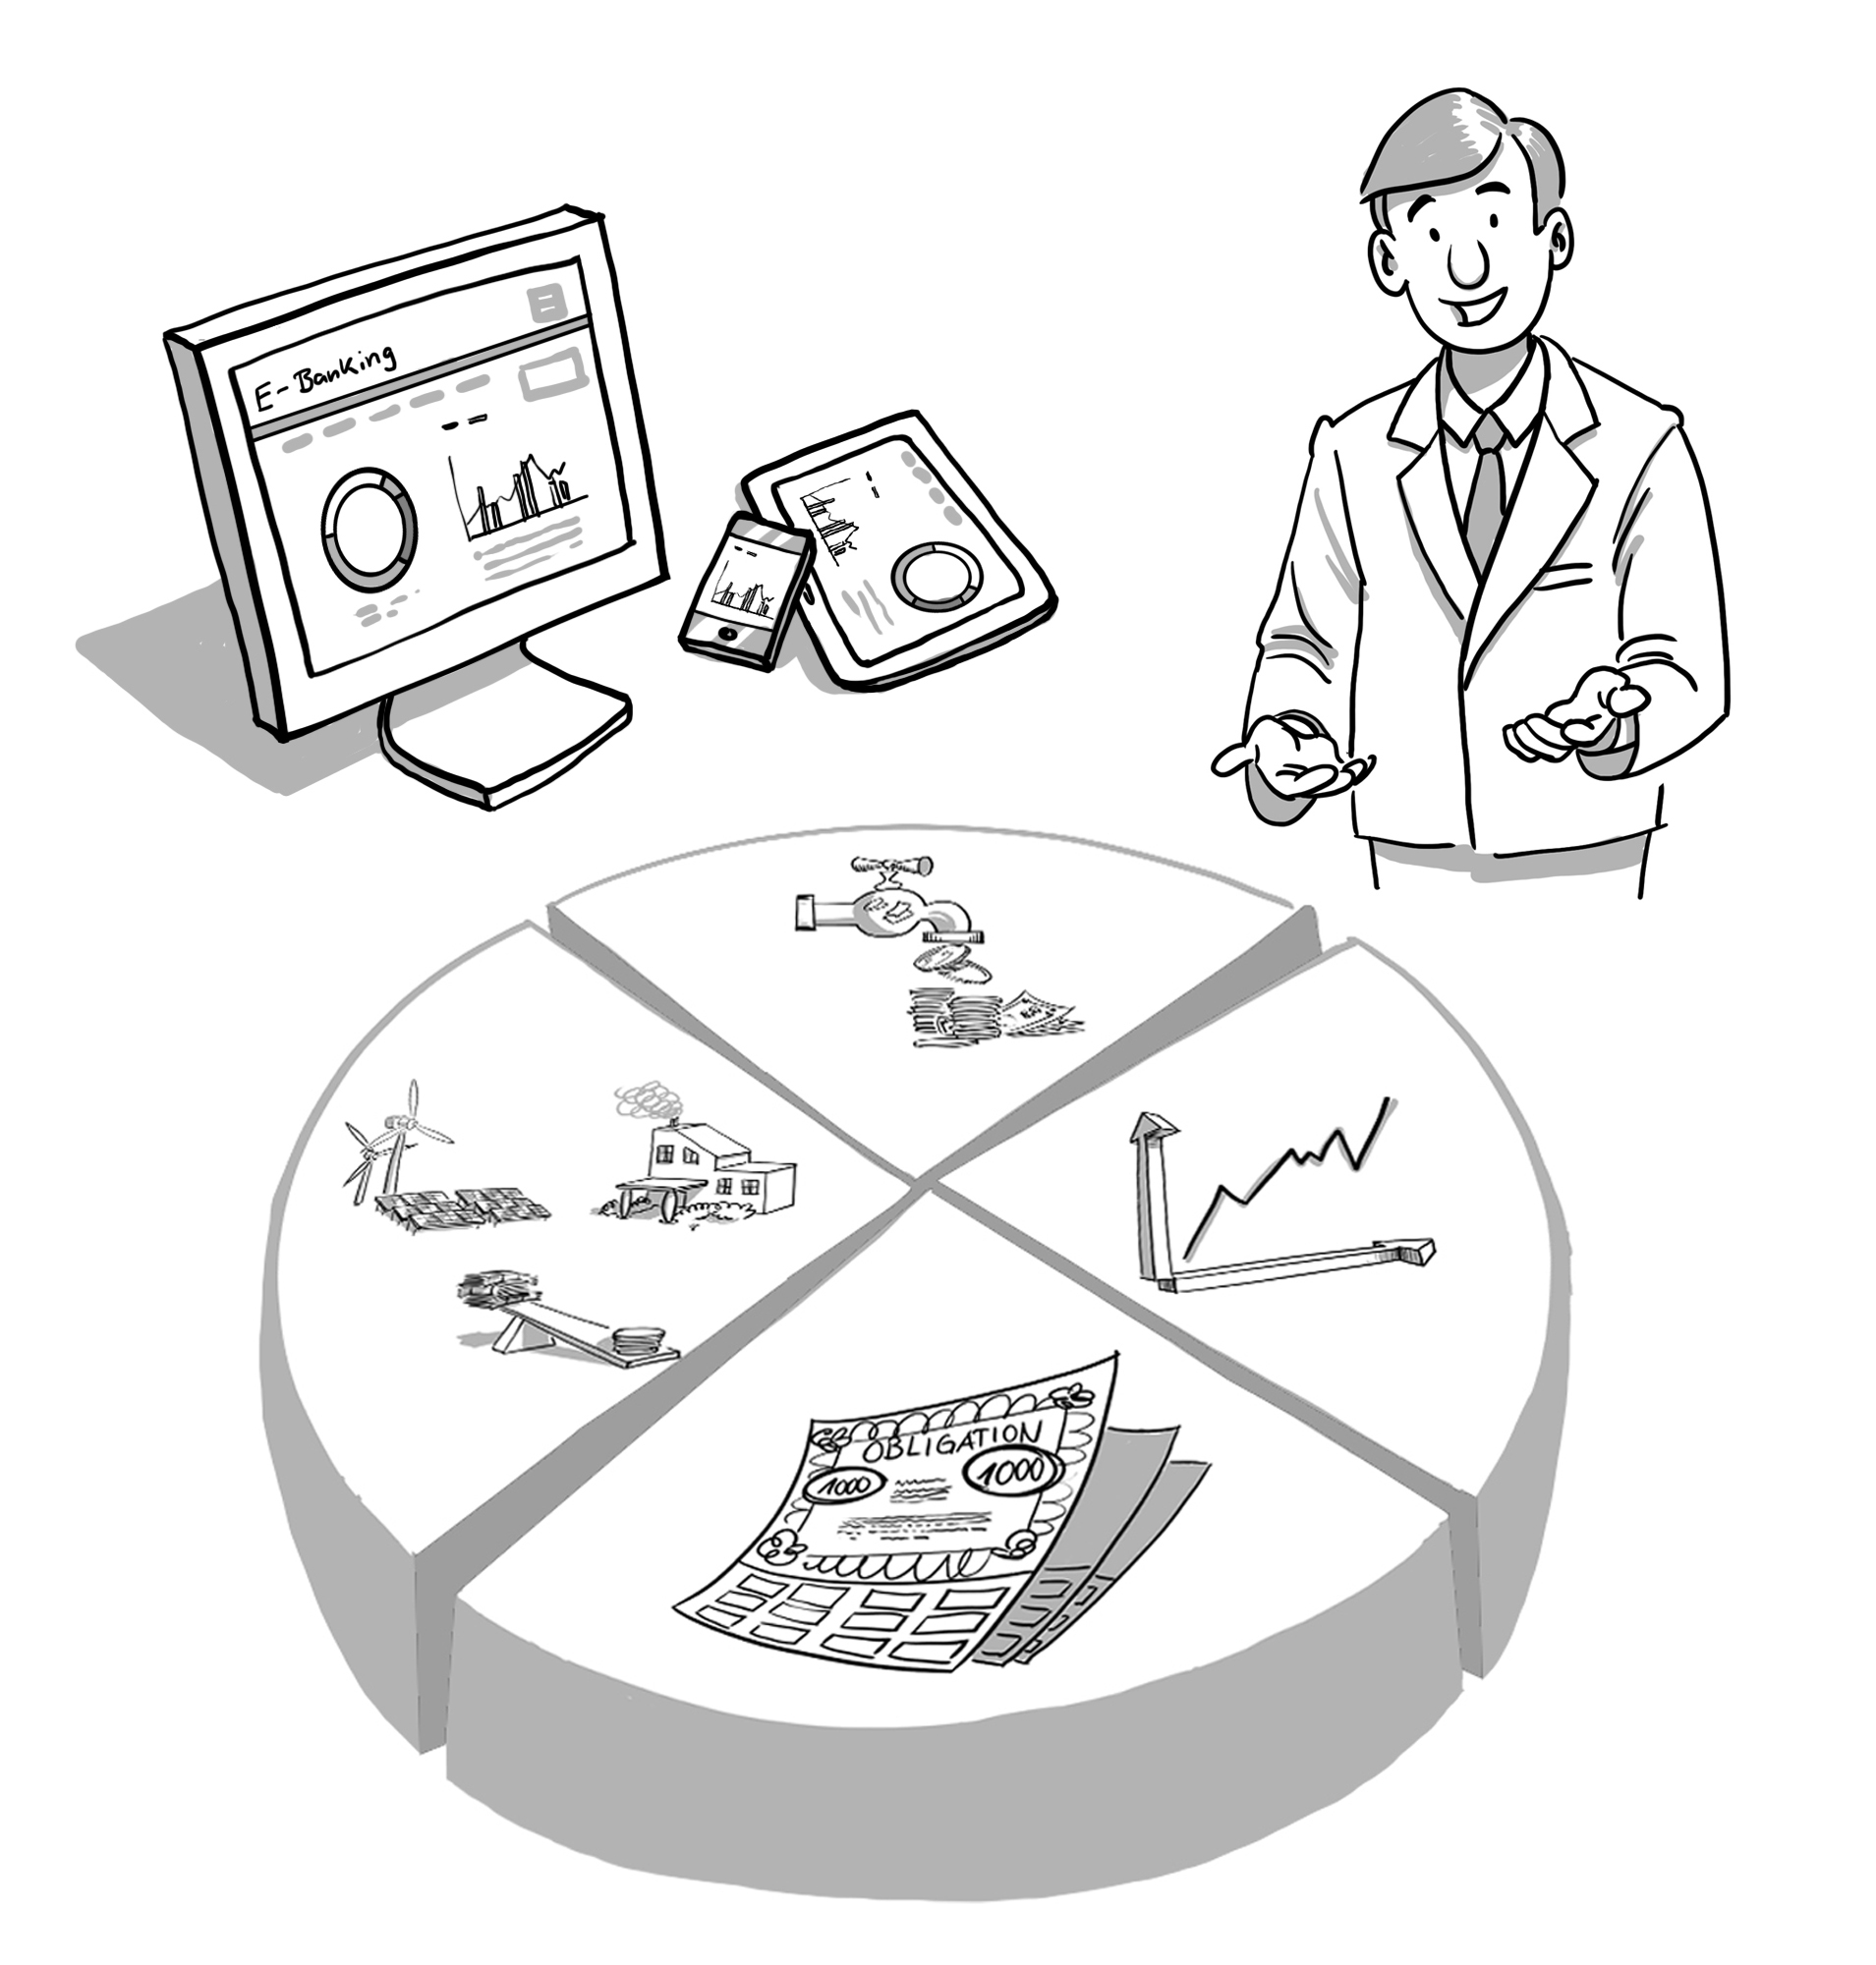
\includegraphics[scale=0.4]{img/InvestmentSolutions.jpg}
	\end{minipage}
\end{figure}

\vspace*{1\baselineskip}

\HRule \\[0.4cm]
{\LARGE \textbf{Development of the Portfolio Management Game}}
\HRule \\[1.5cm]

\vspace*{1\baselineskip}

{\large \textbf{Master Project}}

\vspace*{1\baselineskip}

\scshape % Small caps
\large University of Zurich - Department of Banking and Finance \\ \vspace{3.5mm}

\vspace*{0.5\baselineskip}



\begin{align*}
\textbf{Authors:} &\ \text{Roland Schläfli - roland.schlaefli@gmail.com} \\
&\ \text{Pascal Zehnder - pascal\_zehnder@outlook.com} \\
\textbf{Supervisor:} &\ \text{Prof. Chat Wachamaraontham} \\
\end{align*}

\endgroup
\end{titlepage}

\newpage

\pagenumbering{roman}

% ----------------------------------------
% Inhaltsübersicht
% ----------------------------------------
\tableofcontents

\newpage

% ----------------------------------------
% Start des eigentlichen Inhalts
% ----------------------------------------
\pagestyle{headings}
\pagenumbering{arabic}

\section{Motivation}
\label{sec:motivation}

Students in the field of Banking and Finance at the University of Zurich learn a lot about asset management as well as business management aspects during various courses. In order to give students an opportunity to apply their knowledge and understanding of the portfolio management process, a Portfolio Management Game is used within a seminar for Master students. According to the Department of Banking and Finance, the main targets of this simulation are the following learning outcomes:
\begin{itemize}
  \item Students learn how money can be systematically invested in financial markets.
  \item Students learn what factors make financial market forecasts possible and what limitations the models have for forecasting.
  \item Students learn which factors are relevant for the success (performance) of investments and can distinguish between factors that promise short-term success and aspects that are relevant in the long term.
\end{itemize}

In the simulation, the students act in groups as heads of a bank’s portfolio management and are responsible for both the investment strategy and the business management of investment funds. The games content focuses on a structured investment process, which covers the steps from getting to know different customer types of the bank, selecting a suitable long-term Strategic Asset Allocation, adjust it according to the status of the economy for the Tactical Asset Allocation and select appropriate titles for the depot realization. Competition for better performance for their clients among the different student teams makes the learning process entertaining.

\begin{figure}[h!]
  \centering
  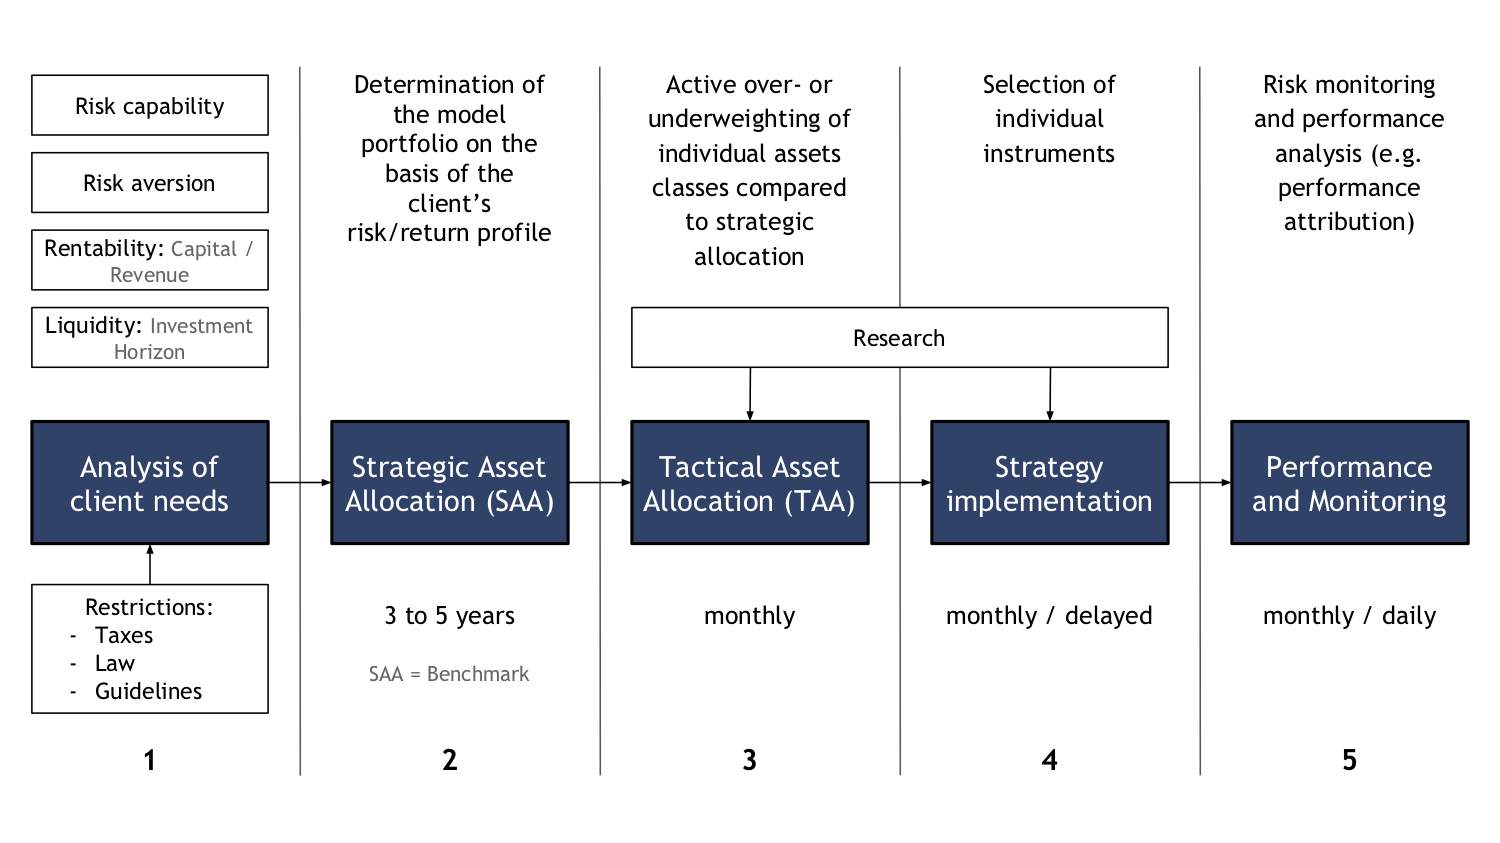
\includegraphics[scale=0.6]{img/private_banking_process.png}    \caption{Investment process}
\end{figure}

However, the currently used version of the Portfolio Management Game is technically and didactically outdated. The currently used Portfolio Management Game (Portfoliomanagement SIM) was initially developed in 2005 by the Department of Banking and Finance at the University of Zurich in cooperation with the Swiss bank Julius Bär as well as game solution ag. A rapid technological development since that time allows new perspectives and possibilities in the field of game-based learning.\\

% TODO insert old game screenshots? not sure if helpful

This project aims to redesign and reprogram the existing Portfolio Management Game so that it is up to date both from a content, technical and didactic point of view. Therefore, a project team from the Department of Banking and Finance and Department of Informatics have decided to cooperate on a modern version of the Portfolio Management Game. From the content side, a project team around Prof. Dr. Markus Leippold and Dr. Benjamin Wilding have been assembled. From the IT side, Prof. Dr. Chat Wacharamanotham together with two students (also the authors of this work) are in the lead. Both student members of the project team work at the Department of Banking and Finance UZH as web developers parallel to their studies achieving their Master’s degree in Informatics. Both interested in developing applications from scratch and analyzing the procedure of financial processes. By re-developing the application the Department of Banking and Finance wants to achieve a sustainable simulation of a typical portfolio management process. The simulation should help the students within their learning process by focussing on practical decision making, building up on their theoretical knowledge. \\

The present work focuses more on the IT side of the project. Subsequently, a more detailed description of the project scope is provided.

\section{Project Description}
The ''Portfolio Management Game'' was initially developed in 2001 by an external company for the Department of Banking and Finance. This simulation of a portfolio manager was being used from the DBF over several years by multiple seminars of their departement. A course named ''Advanced Portfolio Seminar'' has given insights to the portfolio management process for Master students by playing the game in between different rounds playing the game. For the final seminar of the ''Executive Education'' the game was being played for two days on Uetliberg with all the executive students.

The game has been deprecated by its implemented technologies and after each round the supervisors had to collect a USB-stick where all decisions of the students have been saved to. The supervisors had to collect this data for each group on a central device with administrative access (on a windows native application) to calculate the result of the teams decisions.

\section{Procedure}

\subsection{Basic Requirements Engineering}
User stories

\subsection{Student Observation}

\subsection{Implementation}
Iterative Prototyping

\section{Architecture}

\begin{center}
  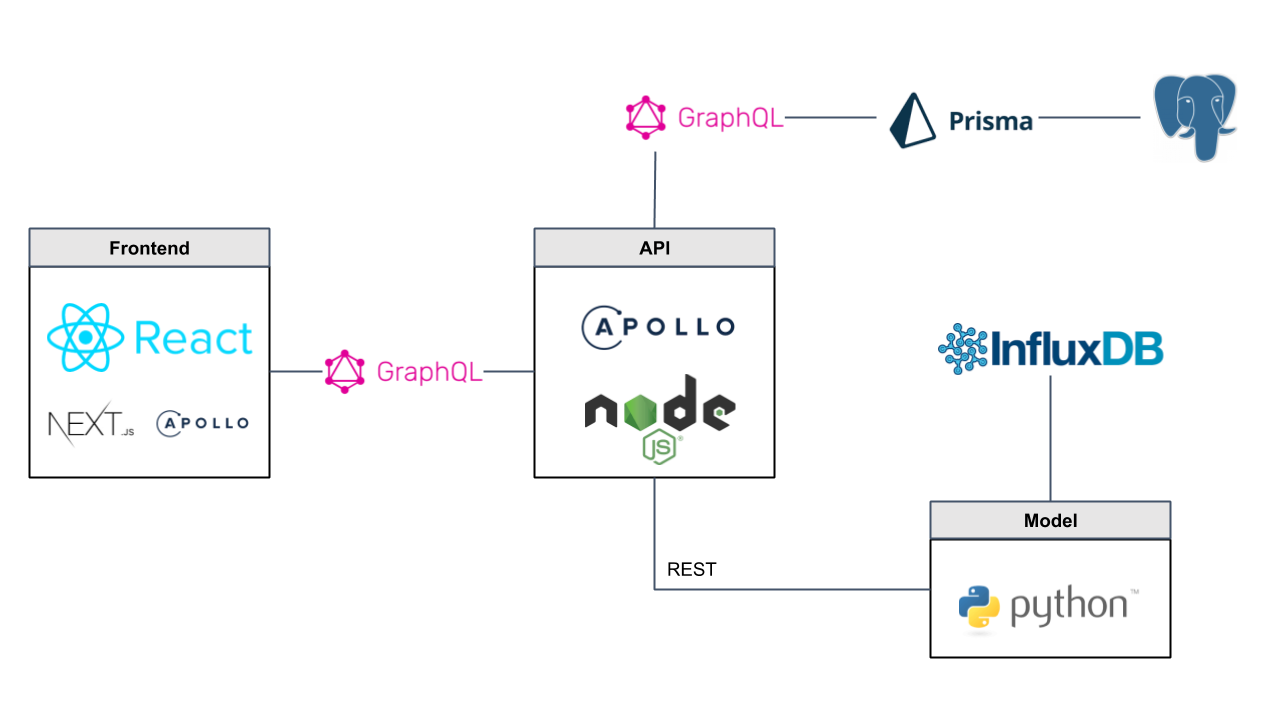
\includegraphics[scale=0.45]{img/architecture.png}
\end{center}

\subsection{Frontend}
We use the React Framework which is developed by Facebook. Based on NextJS.

\subsection{API}
Bla


\subsection{Model}
All calculations of the simulation are performed in a python-model which interacts with the time series data stored on an InfluxDB. A Restful service fetches the data from the model.

\subsection{Contnious development}

\section{Application Overview}

\subsection{Architecture}

\begin{center}
  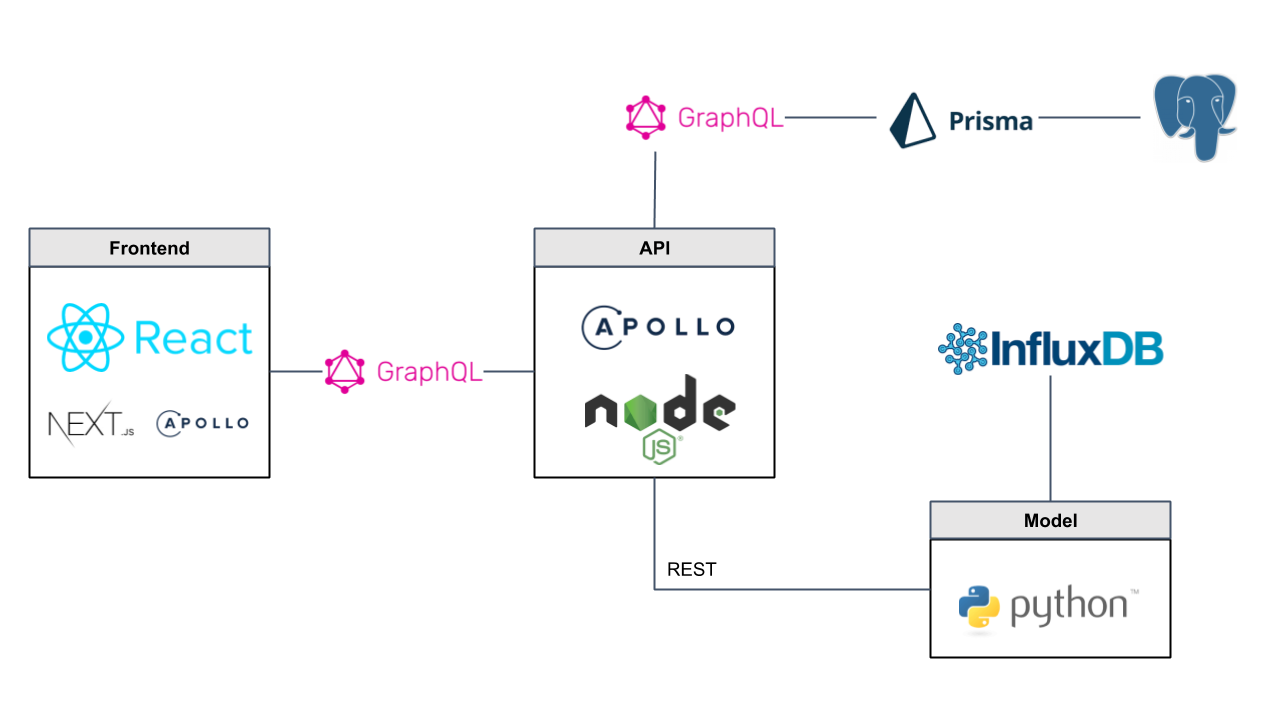
\includegraphics[scale=0.45]{img/architecture.png}
\end{center}

\subsubsection{Frontend}
We use the React Framework which is developed by Facebook. Based on NextJS.

\subsubsection{API}
Bla


\subsubsection{Model}
All calculations of the simulation are performed in a python-model which interacts with the time series data stored on an InfluxDB. A Restful service fetches the data from the model.

\subsection{Administration}

\subsection{Team View}

\section{Future Development}



\newpage

% ----------------------------------------
% Literaturverzeichnis
% ----------------------------------------
\selectlanguage{ngerman}
\bibliography{bachelor_thesis}


\end{document}
